% Auto-generated by the analysis pipeline — do not edit
% y > 0: Overreacts  |  y < 0: Underreacts
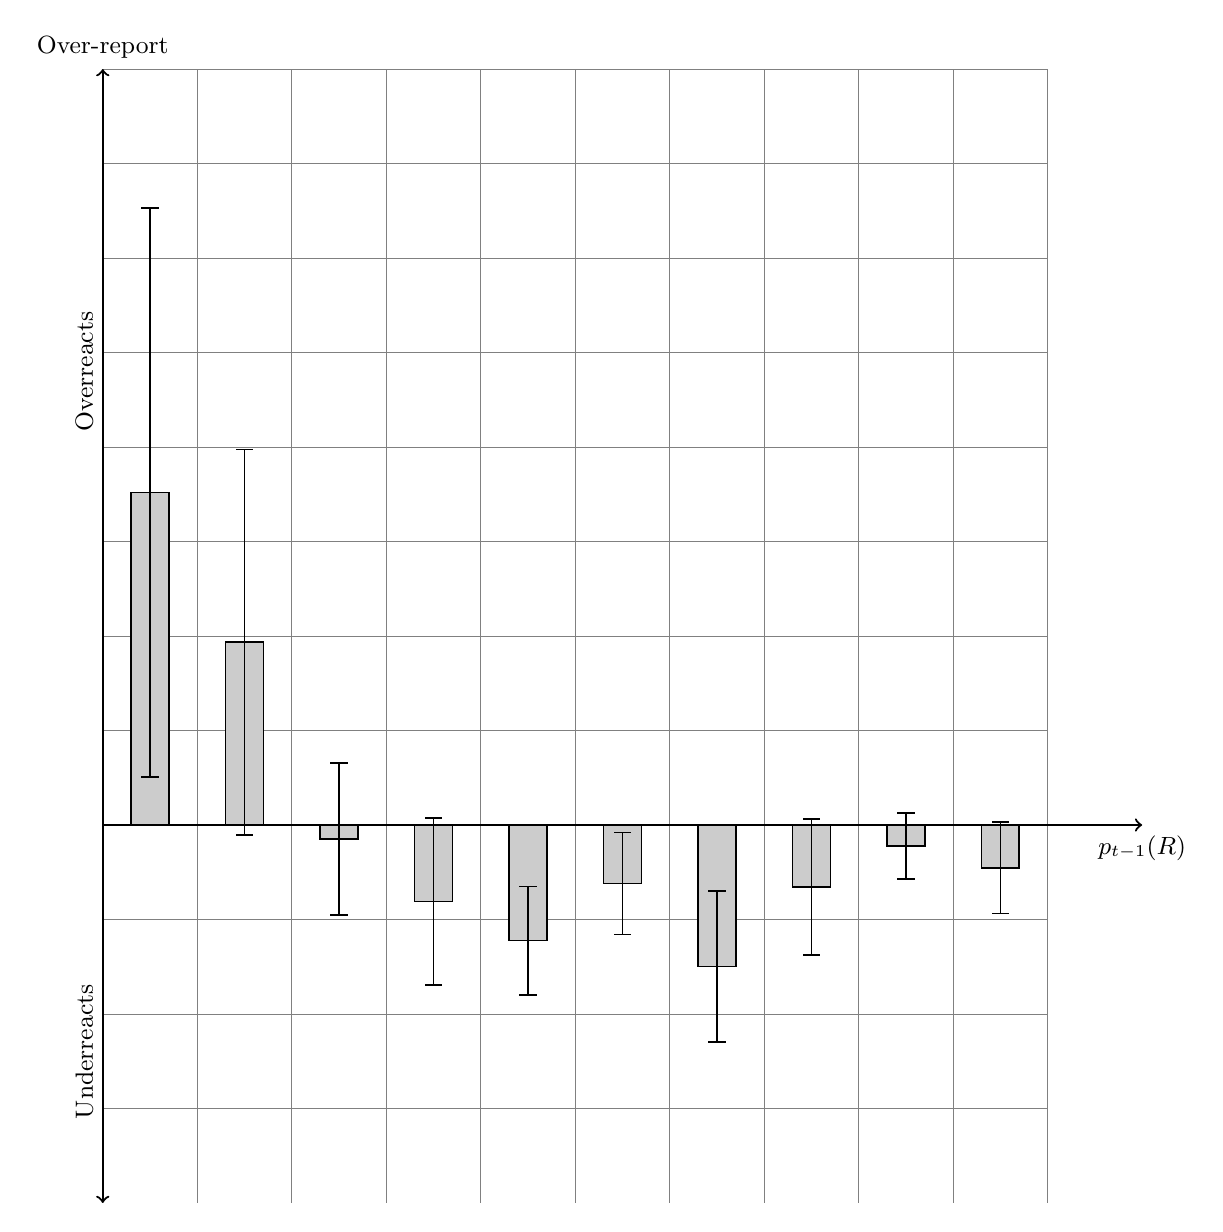
\begin{tikzpicture}[scale=12]
\draw[help lines,step=0.1] (0,-0.4) grid (1,0.8);
\filldraw[opaque,white!80!black] (0.03,0) rectangle (0.07,0.3519);
\draw[line width=0.6] (0.03,0) rectangle (0.07,0.3519);
\draw[line width=0.6,|-|] (0.05,0.0501) -- (0.05,0.6538);
\filldraw[opaque,white!80!black] (0.13,0) rectangle (0.17,0.1935);
\draw[line width=0.6] (0.13,0) rectangle (0.17,0.1935);
\draw[line width=0.6,|-|] (0.15,-0.0114) -- (0.15,0.3983);
\filldraw[opaque,white!80!black] (0.23,0) rectangle (0.27,-0.0149);
\draw[line width=0.6] (0.23,0) rectangle (0.27,-0.0149);
\draw[line width=0.6,|-|] (0.25,-0.0963) -- (0.25,0.0665);
\filldraw[opaque,white!80!black] (0.33,0) rectangle (0.37,-0.0809);
\draw[line width=0.6] (0.33,0) rectangle (0.37,-0.0809);
\draw[line width=0.6,|-|] (0.35,-0.1699) -- (0.35,0.0082);
\filldraw[opaque,white!80!black] (0.43,0) rectangle (0.47,-0.1224);
\draw[line width=0.6] (0.43,0) rectangle (0.47,-0.1224);
\draw[line width=0.6,|-|] (0.45,-0.1806) -- (0.45,-0.0642);
\filldraw[opaque,white!80!black] (0.53,0) rectangle (0.57,-0.0619);
\draw[line width=0.6] (0.53,0) rectangle (0.57,-0.0619);
\draw[line width=0.6,|-|] (0.55,-0.1166) -- (0.55,-0.0071);
\filldraw[opaque,white!80!black] (0.63,0) rectangle (0.67,-0.1496);
\draw[line width=0.6] (0.63,0) rectangle (0.67,-0.1496);
\draw[line width=0.6,|-|] (0.65,-0.2304) -- (0.65,-0.0689);
\filldraw[opaque,white!80!black] (0.73,0) rectangle (0.77,-0.0657);
\draw[line width=0.6] (0.73,0) rectangle (0.77,-0.0657);
\draw[line width=0.6,|-|] (0.75,-0.1384) -- (0.75,0.0070);
\filldraw[opaque,white!80!black] (0.83,0) rectangle (0.87,-0.0224);
\draw[line width=0.6] (0.83,0) rectangle (0.87,-0.0224);
\draw[line width=0.6,|-|] (0.85,-0.0580) -- (0.85,0.0133);
\filldraw[opaque,white!80!black] (0.93,0) rectangle (0.97,-0.0453);
\draw[line width=0.6] (0.93,0) rectangle (0.97,-0.0453);
\draw[line width=0.6,|-|] (0.95,-0.0944) -- (0.95,0.0038);
\draw[line width=0.8,->]  (0,0) -- (1.1,0) node[below] {\small{$p_{t-1}(R)$}};
\draw[line width=0.8,<->] (0,-0.4) -- (0,0.8) node[above] {\small{Over-report}};
\draw (0,0.48) node[above,rotate=90] {\small{Overreacts}};
\draw (0,-0.24) node[above,rotate=90] {\small{Underreacts}};
% ADD THEORY CURVE BELOW
\end{tikzpicture}
